\documentclass{standalone}
\usepackage{tikz,tkz-euclide}
\usepackage{ctex}
\setCJKmainfont{Noto Serif CJK SC}
\usepackage{mhchem,siunitx}
\usetikzlibrary{patterns,patterns.meta,calc}
\usetikzlibrary {decorations.pathmorphing, decorations.pathreplacing, decorations.shapes}
\newcommand{\VTube}[3][]{
  \begin{scope}[#1]
    \draw[fill=darkgray](-0.2,#2-0.48)rectangle++(0.78,0.07);
    \draw[fill=brown](0.58,#2-0.48)rectangle++(0.3,0.07);
    \fill[cyan!40!white,fill opacity=0.5](-0.15,#3)--(-0.15,0)arc(180:360:0.15)--(0.15,#3)--cycle;
    % \fill[left color=gray,right color=gray,middle color=white](-0.15,#2-0.15)rectangle++(0.3,0.25);
    \draw[fill=cyan!20!white,fill opacity=0.2](-0.2,#2)arc(90:0:0.05)--(-0.15,0)arc(180:360:0.15)--(0.15,#2-0.05)arc(180:90:0.05)--cycle;
    \draw[fill=brown](-0.22,#2-0.5)rectangle++(0.8,0.07);
    \draw[lightgray,semithick](0.25,#2-0.5)--++(0.02,0.07)arc(180:0:0.01)(0.25,#2-0.5)arc(0:-180:0.01)(0.5,#2-0.5)--++(0,0.07);
  \end{scope}
}
\newcommand{\thermometer}[3][]{
  \begin{scope}[#1]
    \draw(-0.02,#3)arc(180:0:0.02)--(60:0.04)arc(60:-240:0.04)--cycle;
    \draw[semithick,red](0,0)--++(0,#2);
    \fill[red](0,0)circle(0.03);
  \end{scope}
}

\begin{document}
\small
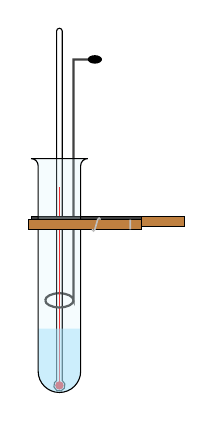
\begin{tikzpicture}[>=stealth,scale=1.8,inner sep=2pt]
  \draw[darkgray,thick](-0.1,0.5)arc(180:0:0.1 and 0.05)--(0.1,2.2)--++(0.2,0);
  \fill(0.25,2.2)ellipse(0.05 and 0.03);
  \thermometer[yshift=-1mm]{1.4}{2.5}
  \draw[darkgray,thick](-0.1,0.5)arc(180:360:0.1 and 0.05);
  \VTube{1.5}{0.3}
\end{tikzpicture}
\end{document}